\documentclass[10pt,a4paper]{article}

\usepackage[utf8]{inputenc}
\usepackage[T1]{fontenc}
\usepackage{lmodern}
\usepackage[margin=1.45cm]{geometry}
\usepackage{graphicx}
\usepackage{xcolor}
\usepackage{booktabs}
\usepackage{tabularx}
\usepackage{array}
\usepackage{enumitem}
\usepackage{multicol}
\usepackage{caption}
\usepackage[hidelinks]{hyperref}

\definecolor{DartsRed}{HTML}{D94F2A}
\definecolor{DartsBlue}{HTML}{2E5BFF}
\definecolor{DartsInk}{HTML}{161616}
\definecolor{DartsMute}{HTML}{5A564E}
\definecolor{DartsPaper}{HTML}{F5F1EA}

\setlength{\parindent}{0pt}
\setlength{\parskip}{0.35em}
\setlist[itemize]{leftmargin=1.15em,itemsep=0.12em,topsep=0.12em}
\setlist[enumerate]{leftmargin=1.35em,itemsep=0.12em,topsep=0.12em}
\captionsetup{font=small,labelfont=bf}
\renewcommand{\arraystretch}{1.08}

\newcommand{\scene}[1]{\textbf{\textcolor{DartsRed}{#1}}}
\newcommand{\metric}[1]{\textbf{\texttt{#1}}}

\title{\vspace{-1.5cm}\textbf{\Huge DArts}\\[0.15em]
\Large Diversity in the MoMA Collection\\[0.35em]
\normalsize COM-480 Data Visualization - Milestone 3 Process Book}
\author{Oussama Ghali (341478) \and Nour Guermazi (314474) \and Isabella Linde (423106)}
\date{May 2026\\
\href{https://com-480-data-visualization.github.io/DArts/}{com-480-data-visualization.github.io/DArts/}\\
\href{https://github.com/com-480-data-visualization/DArts}{github.com/com-480-data-visualization/DArts}}

\begin{document}
\maketitle
\vspace{-0.8em}

\begin{figure}[h]
  \centering
  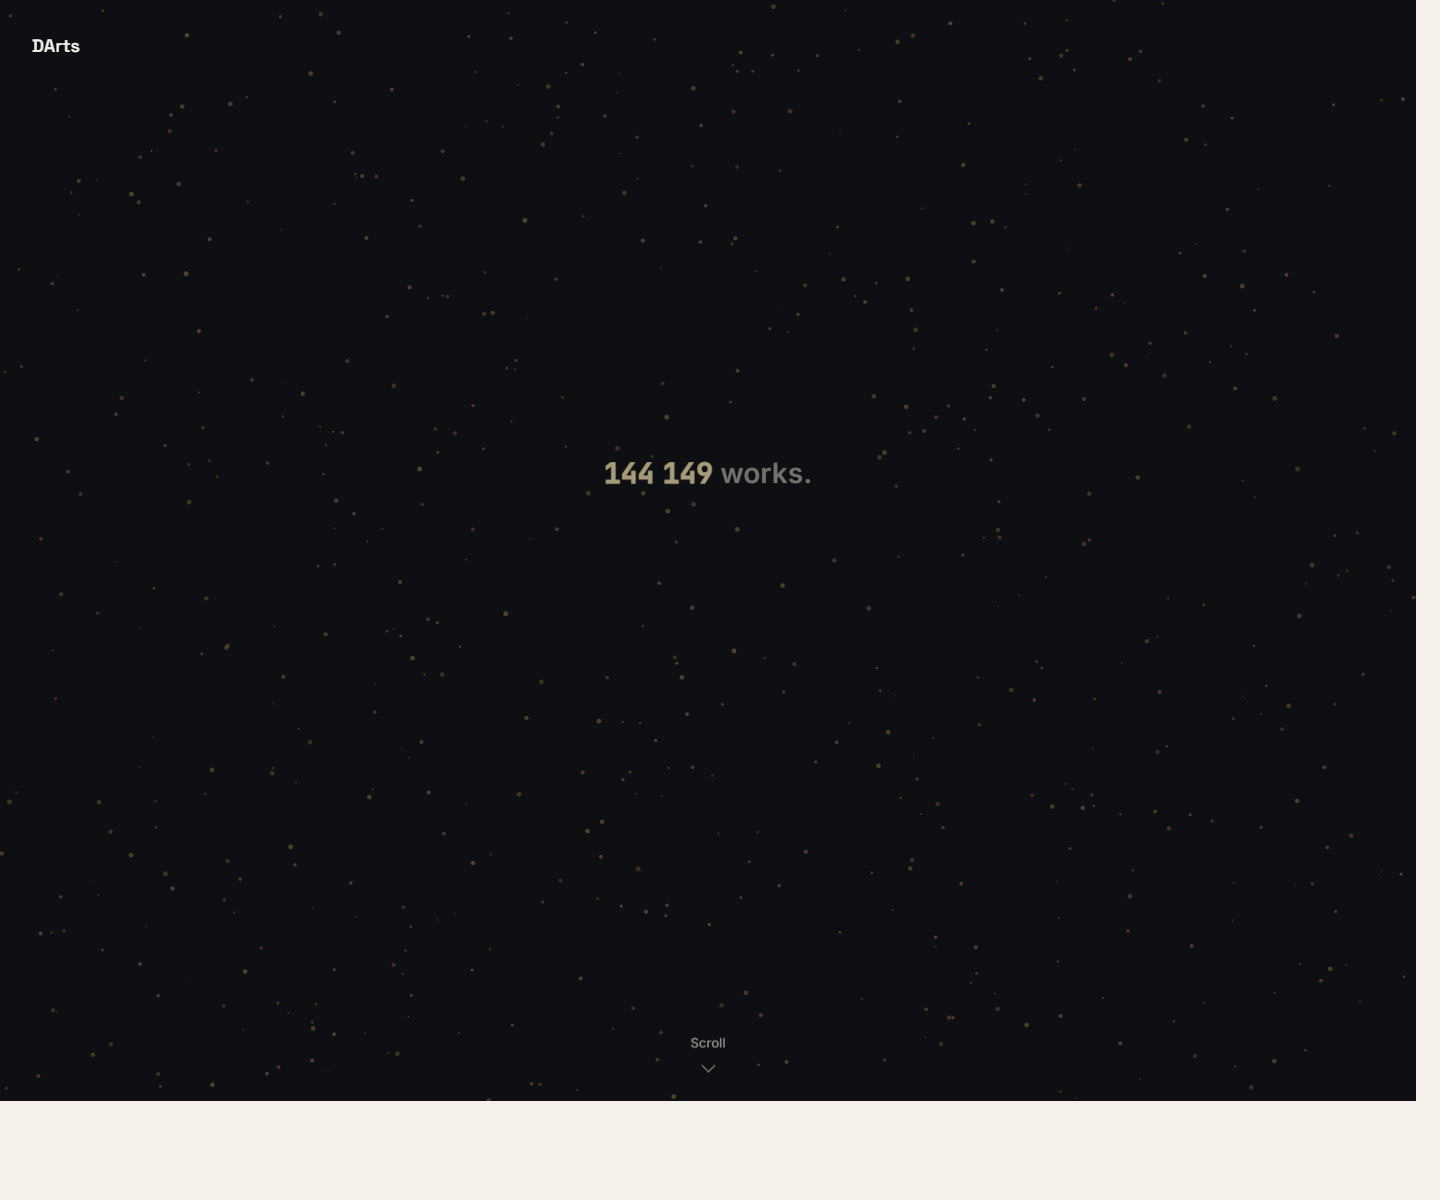
\includegraphics[width=0.86\linewidth]{figures/preview.png}
  \caption{Final DArts site: a scroll-driven narrative moving from collection shape to geography, gender, medium, and a personal artist match.}
\end{figure}

\section*{1. Motivation and Question}
MoMA is often imagined through canonical paintings and sculptures. The recorded collection tells a wider story: works on paper dominate the archive, artist nationality is geographically concentrated, gender representation changes slowly, and representation varies sharply by medium. Our central question is:
\textbf{who is actually present in the recorded MoMA collection, and how does that presence change by medium, place, gender, and time?}

The target audience is broad: general visitors, students, and researchers who may not know art history. We therefore designed DArts as a martini-glass narrative: author-driven scenes establish the main findings, then the medium explorer opens into reader-driven filtering, and the quiz closes with a personal artist match.

\section*{2. Data}
The data source is the public Museum of Modern Art Collection repository. We use the artwork and artist CSV files and aggregate them into compact JSON files before runtime. The final site uses \metric{144,149} cleaned artworks and \metric{11,879} cleaned artists. A permissive date parser extracts the first reliable year between 1700 and 2030, keeping undated records rather than silently dropping them. Countries are mapped through a curated nationality-to-ISO3 lookup and then collapsed to eight UN M49-inspired region buckets.

\begin{table}[h]
\centering
\small
\begin{tabularx}{0.94\linewidth}{>{\bfseries}l r X}
\toprule
Item & Count & Design consequence \\
\midrule
Cleaned artworks & 144,149 & Treemap percentages use the full cleaned corpus. \\
Dated cleaned artworks & 141,884 & Time filters exclude only records that cannot be dated. \\
Cleaned artists & 11,879 & Artist match and country panels remain lightweight. \\
Mapped artist credits & 156,360 & Globe includes an explicit unmapped-nationality note. \\
Unmapped nationality credits & 3,675 & Missing metadata is surfaced, not hidden. \\
\bottomrule
\end{tabularx}
\caption{Reconciliation from \texttt{data/build\_report.txt}.}
\end{table}

\section*{3. Design Process}
The initial sketches explored art-object metaphors: framed works for collection shape, an orthographic globe for origin, layered area/line charts for gender, small multiples for medium, and a hand-drawn quiz card for the personal ending. During implementation we kept the art-world tone but replaced encodings that would be hard to defend in COM-480: pie/donut sketches became 100\% stacked bars, decorative artwork placeholders became metadata cards and MoMA links, and freeform annotations became leader-line callouts tied to data points.

\begin{figure}[h]
\centering
\begin{tabular}{ccc}
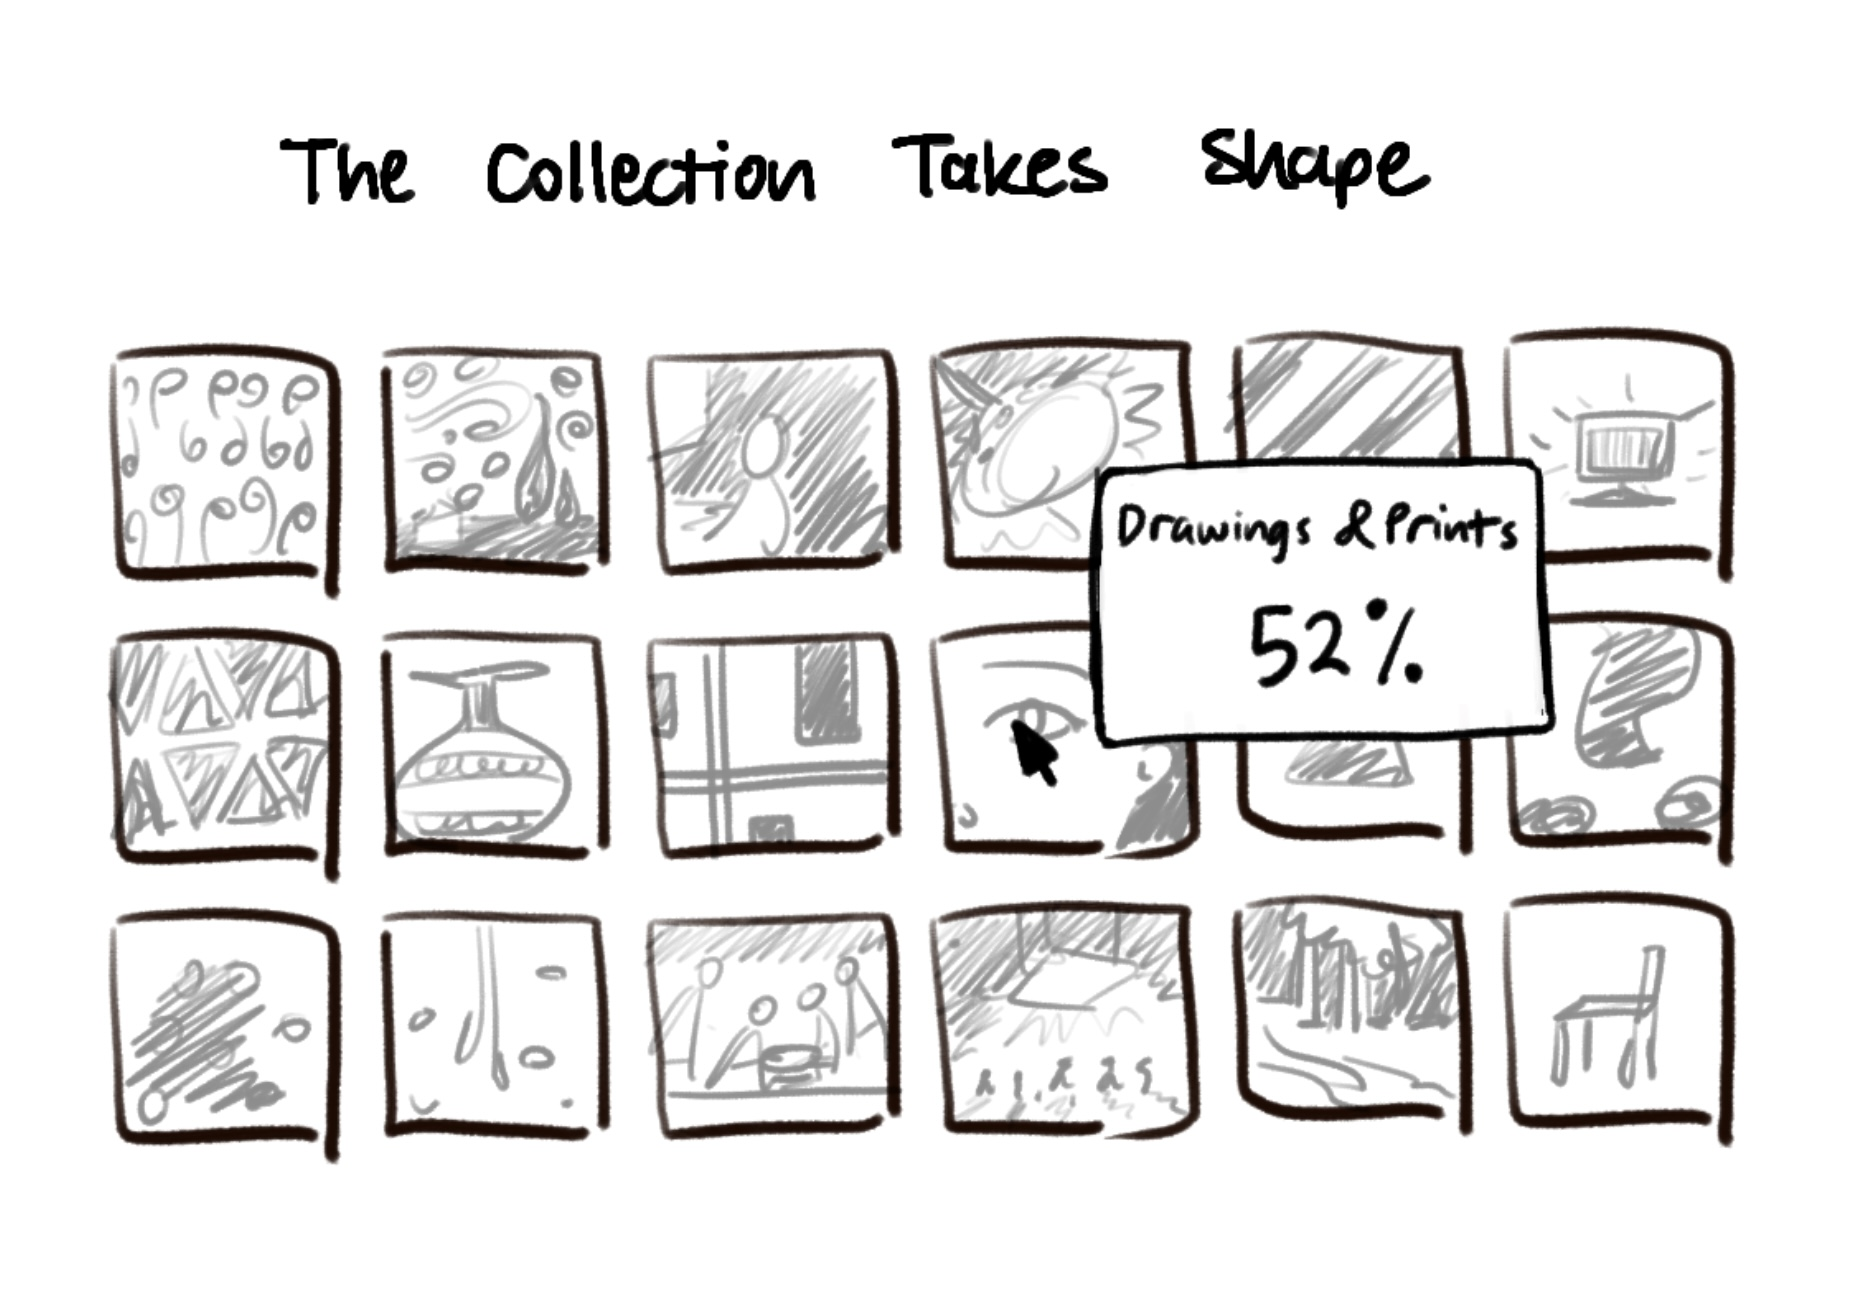
\includegraphics[width=0.29\linewidth]{figures/scene1sketch.jpg} &
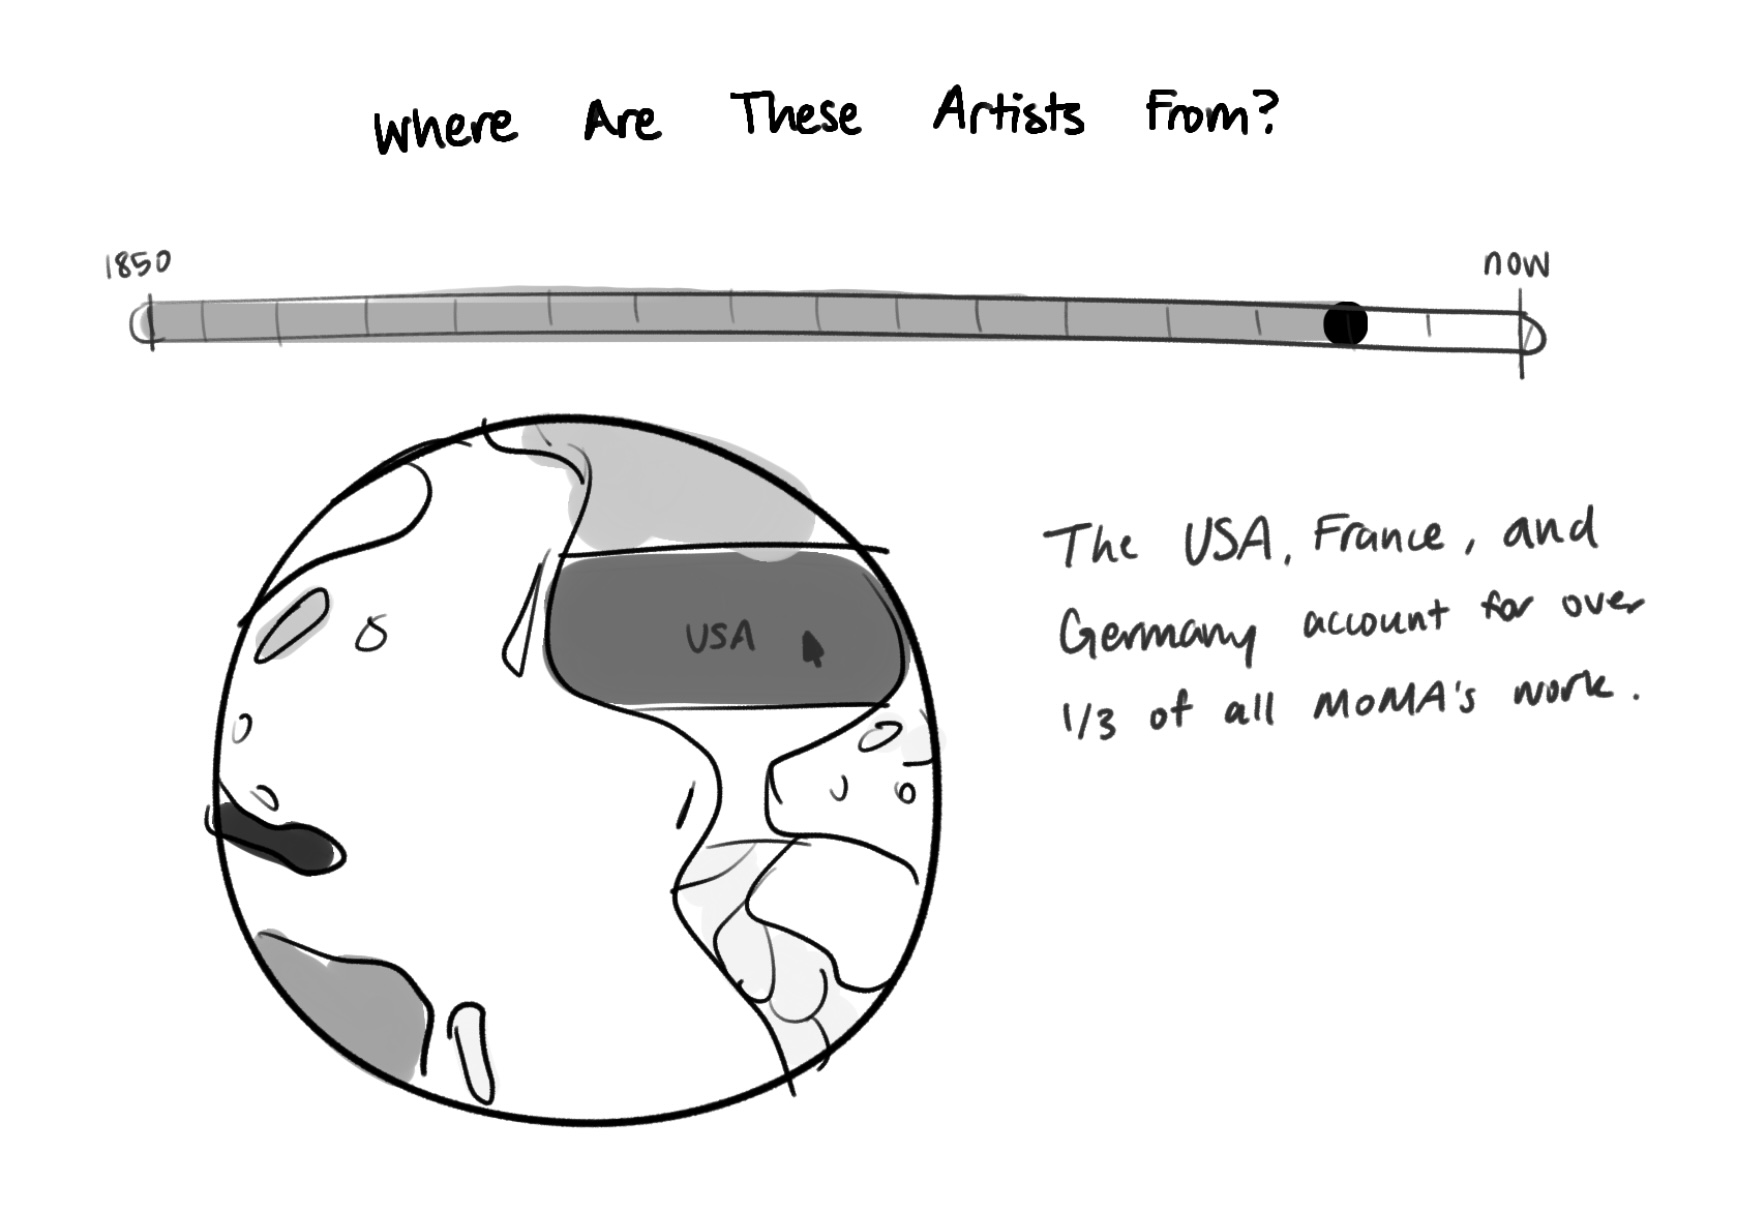
\includegraphics[width=0.29\linewidth]{figures/scene2sketch.jpg} &
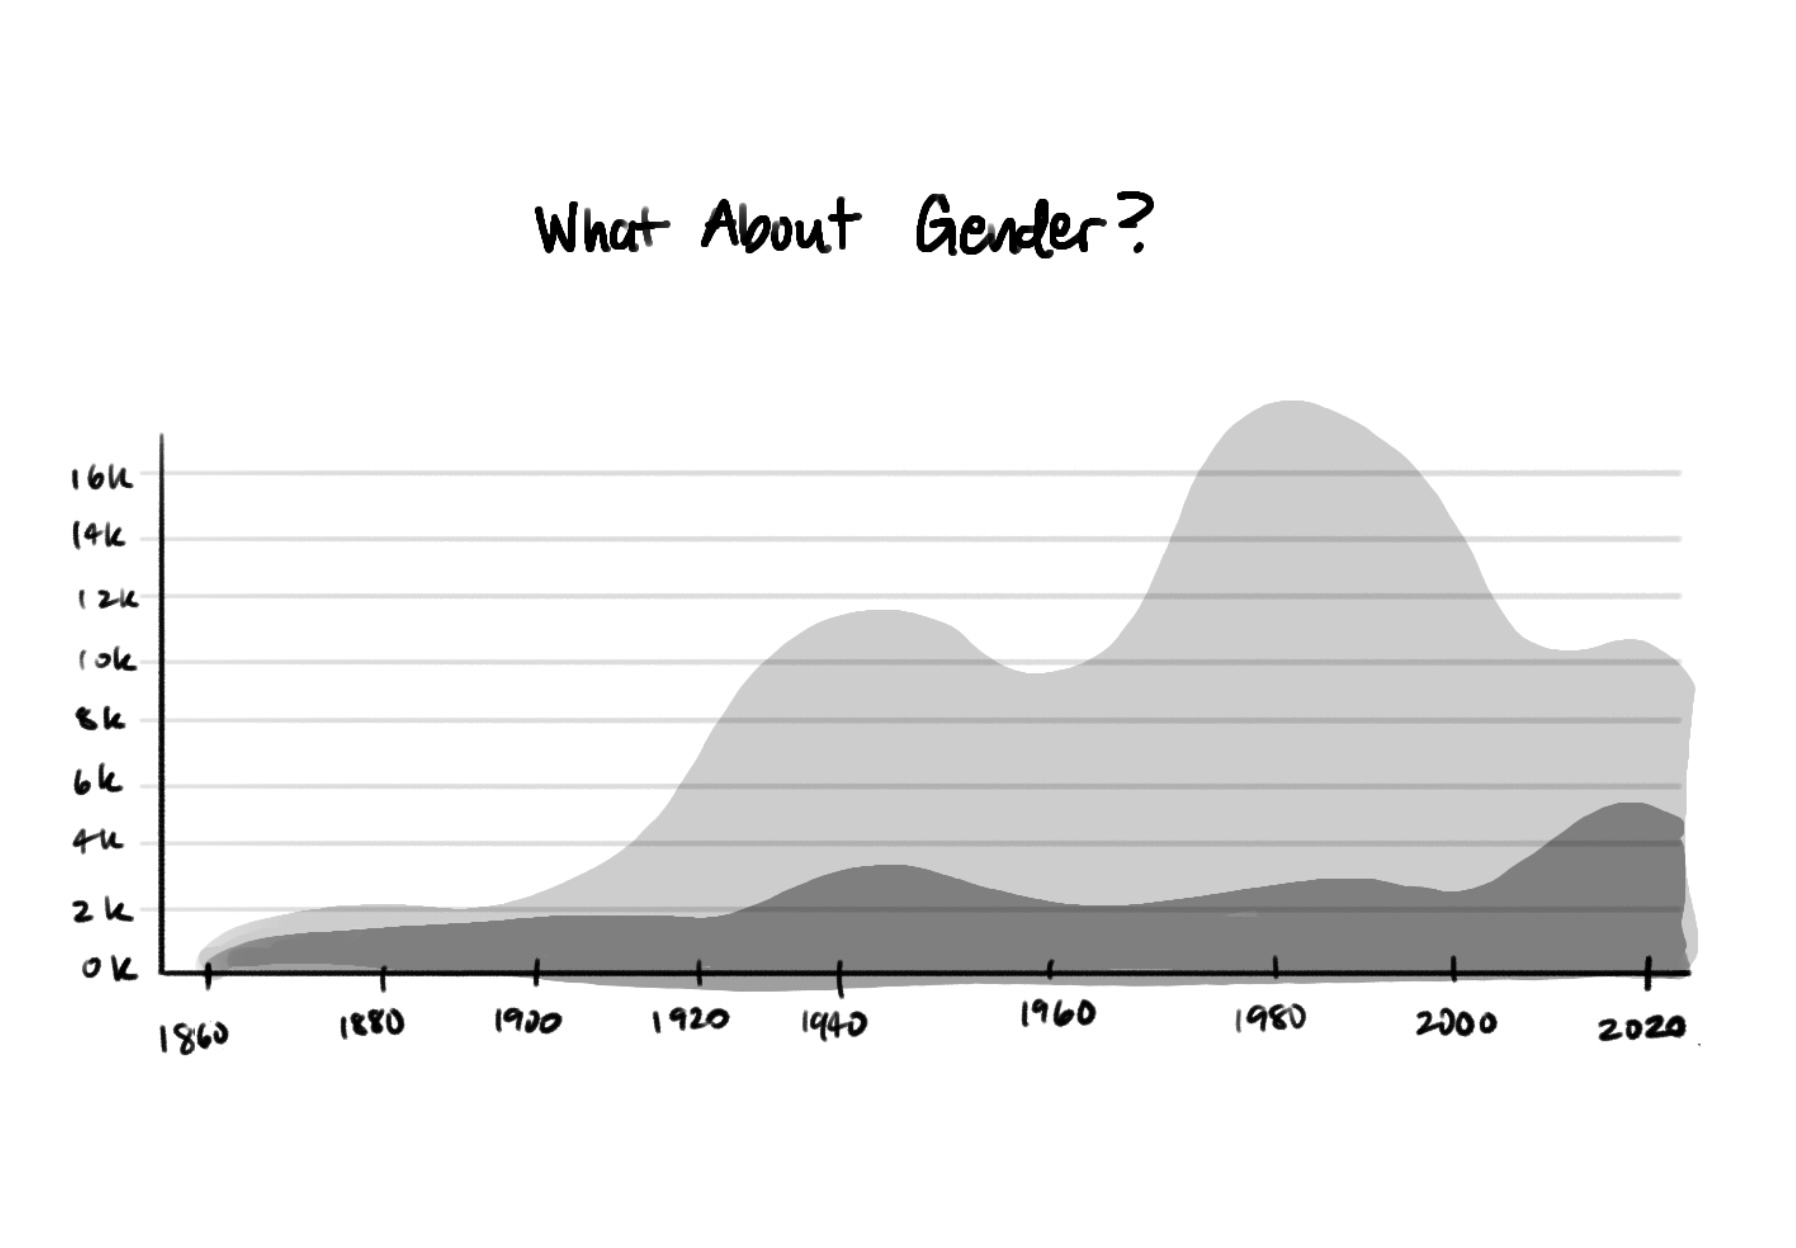
\includegraphics[width=0.29\linewidth]{figures/scene3sketch.jpg} \\
\small Scene 1 sketch & \small Scene 2 sketch & \small Scene 3 sketch \\
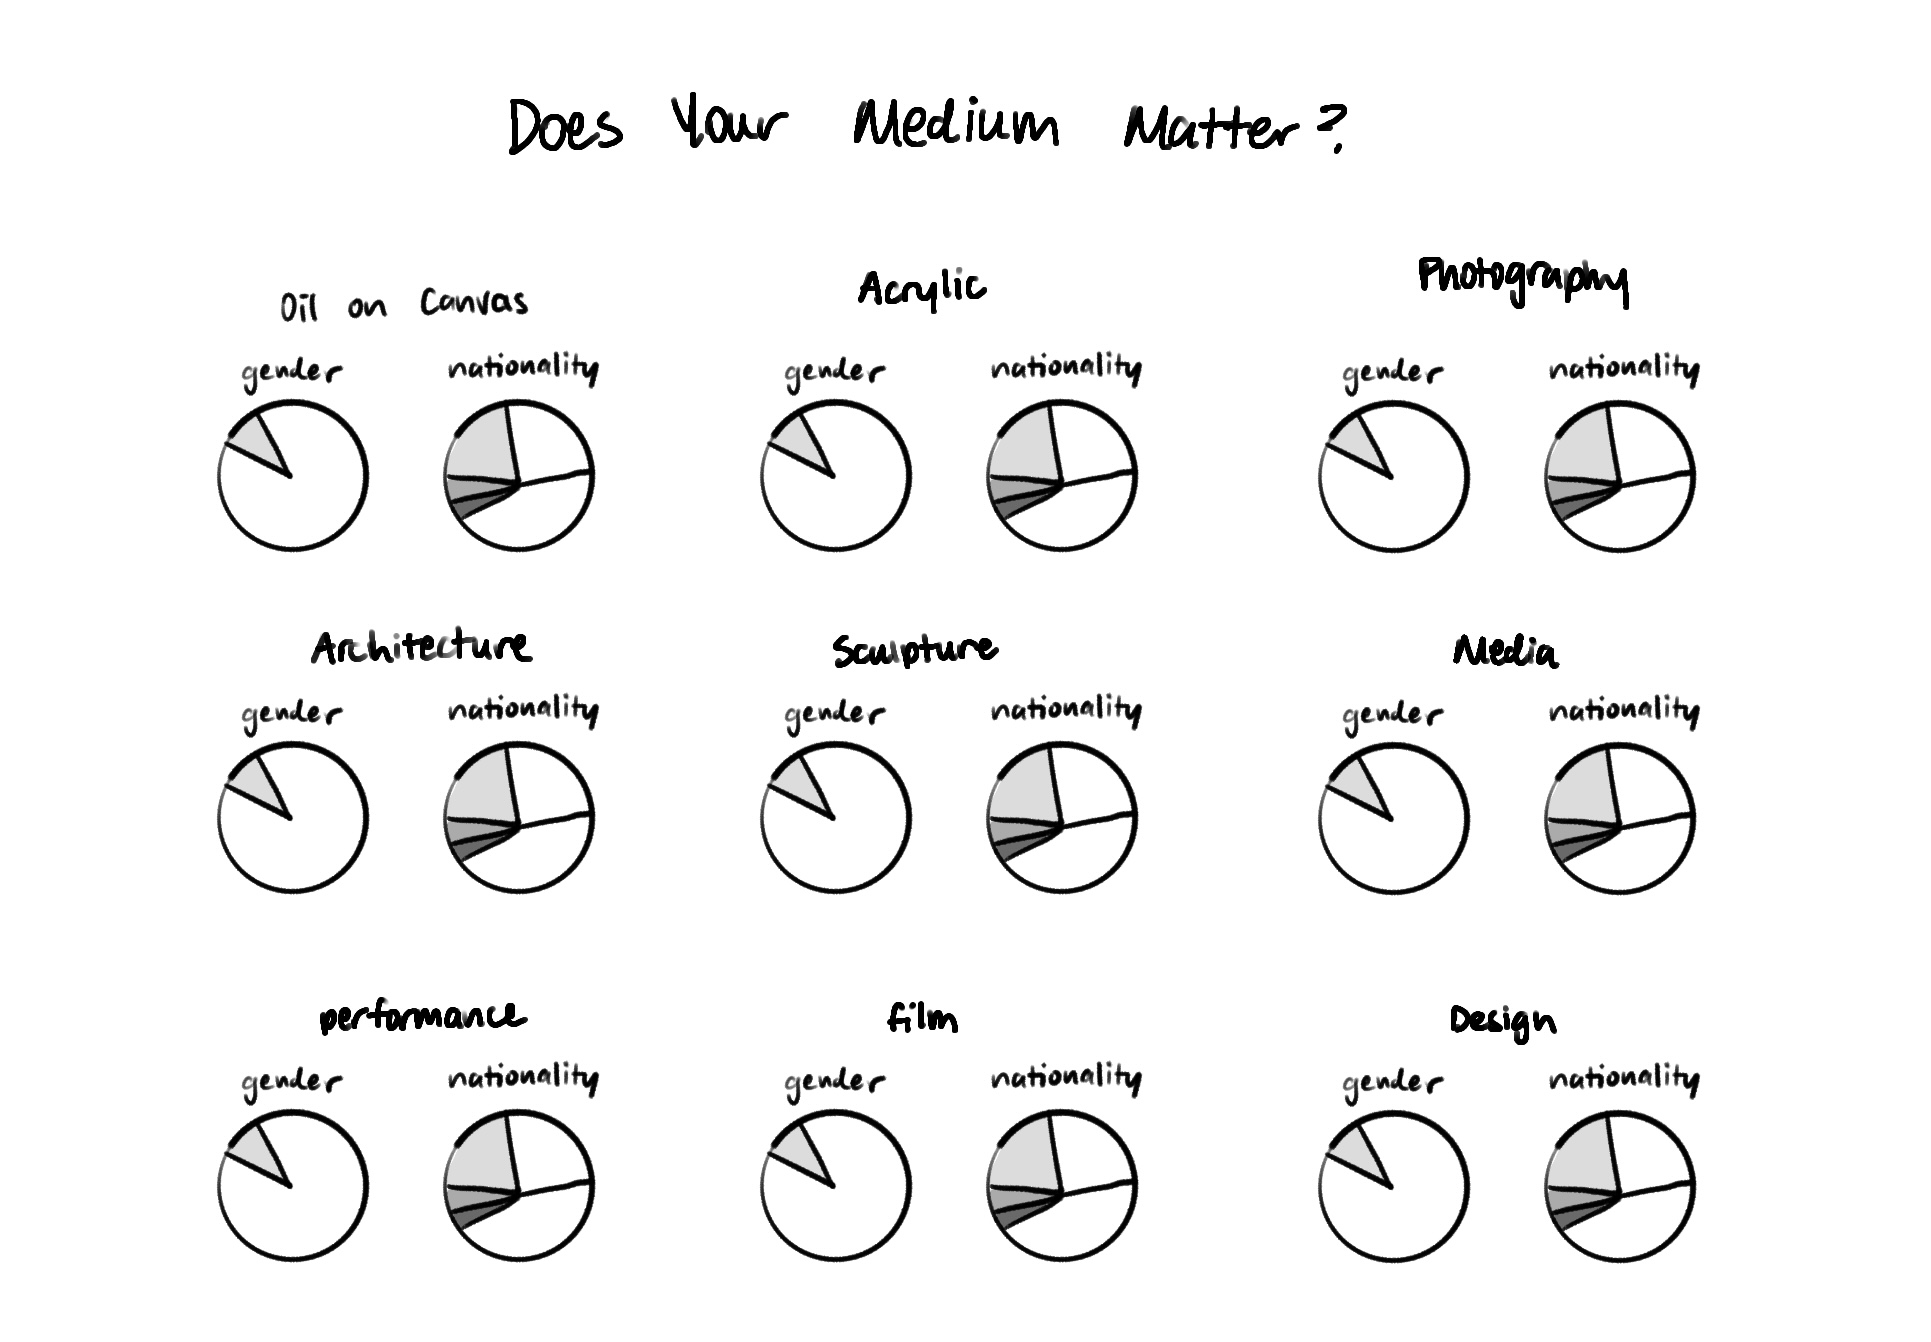
\includegraphics[width=0.29\linewidth]{figures/scene4sketch.jpg} &
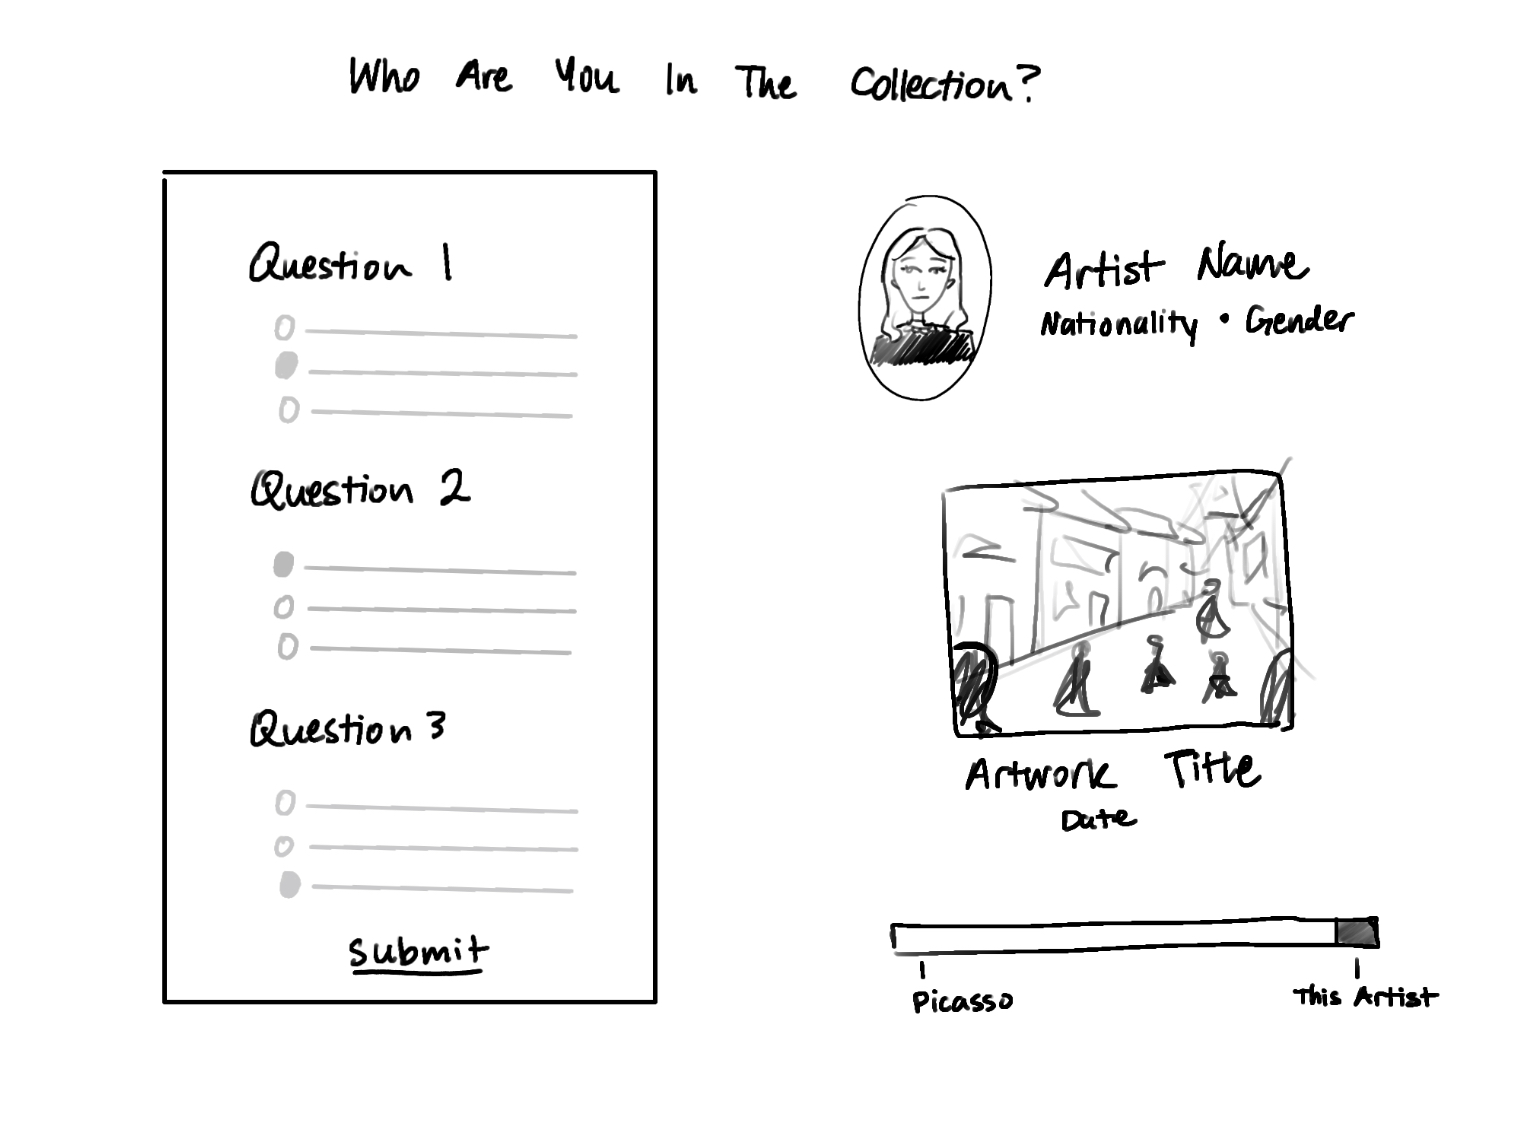
\includegraphics[width=0.29\linewidth]{figures/scene5sketch.jpg} &
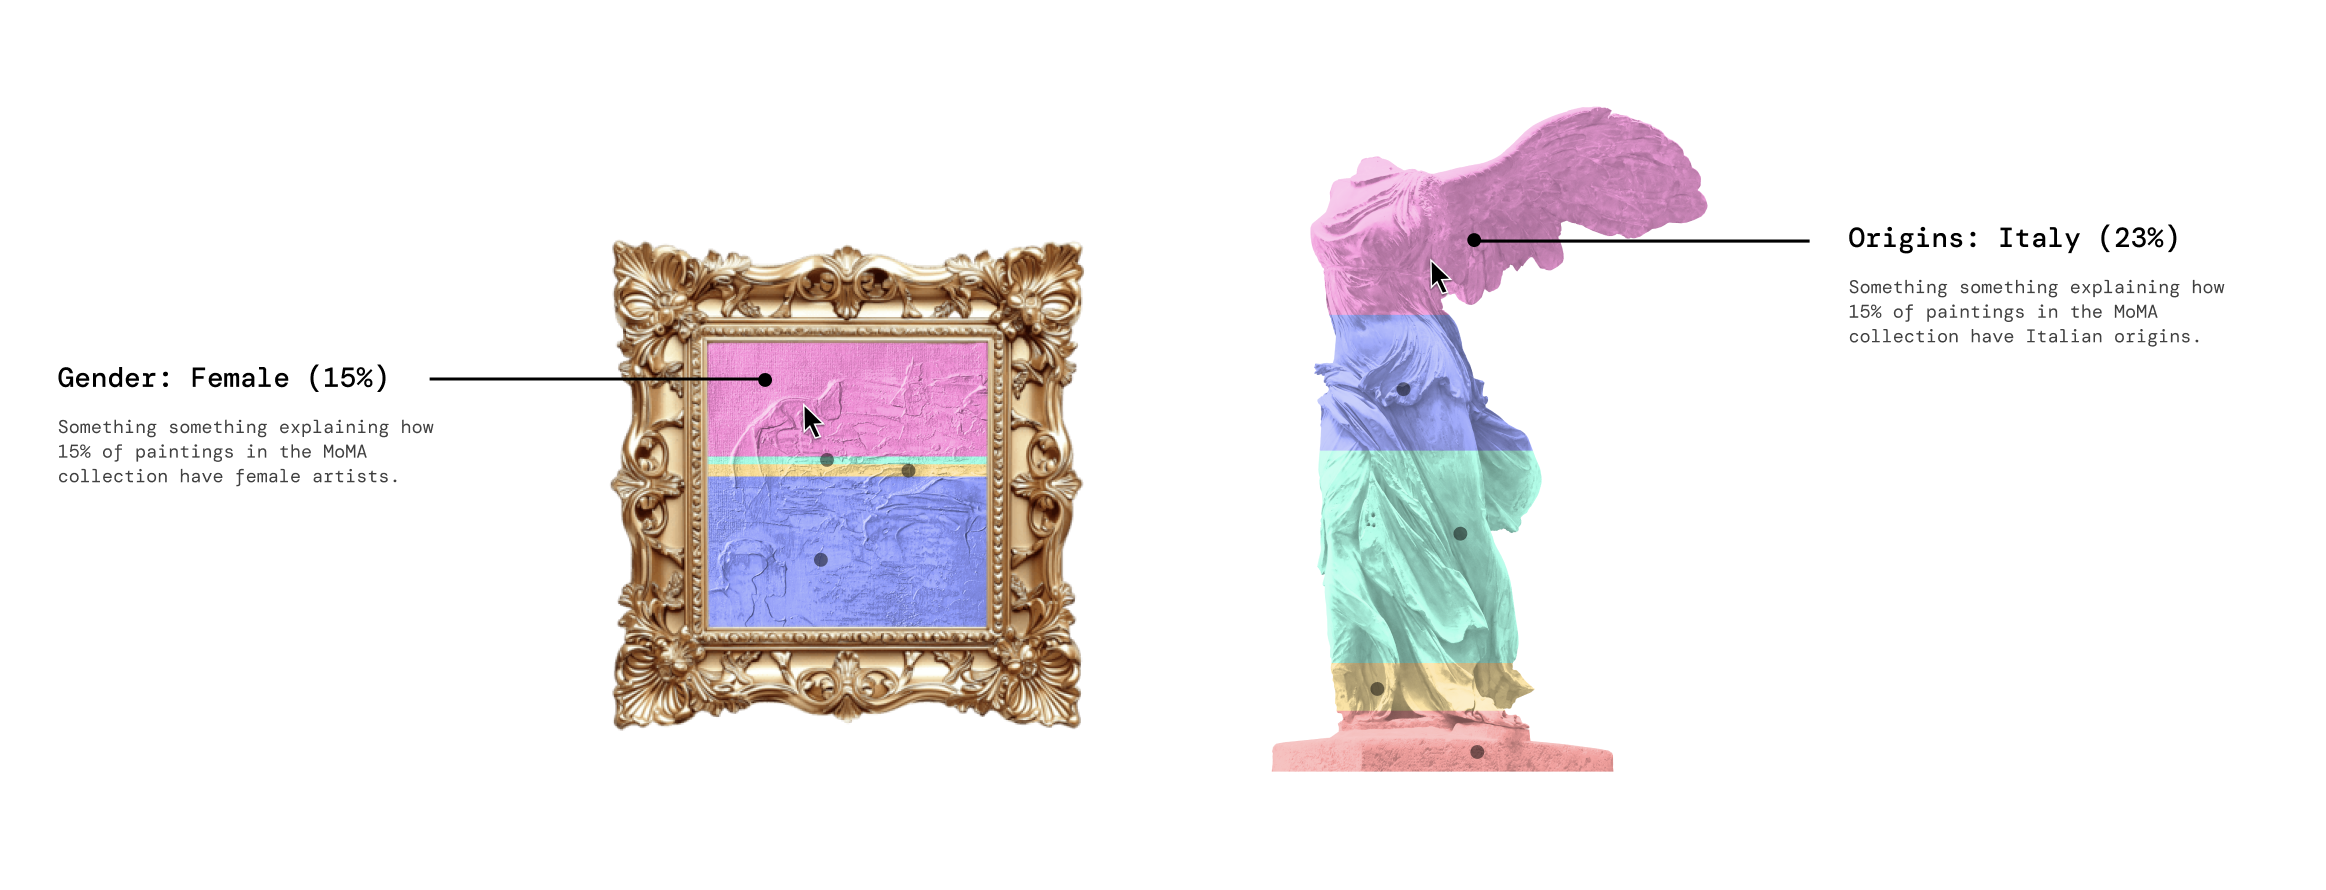
\includegraphics[width=0.29\linewidth]{figures/annotation-sketch.png} \\
\small Scene 4 sketch & \small Scene 5 sketch & \small annotation study
\end{tabular}
\caption{Sketches from M2 and the final design direction. The final site keeps the authored art tone but uses course-defensible marks and channels.}
\end{figure}

\section*{4. Visualization Choices}
\textbf{\scene{Scene 1: The Collection Takes Shape.}} A treemap uses area to encode collection-area size. Area is less precise than common-position encodings, but it is appropriate for a part-to-whole overview with few large categories. One accent color highlights the active claim at a time; all other leaves remain neutral, following Gestalt pop-out and Tufte's data-ink principle.

\textbf{\scene{Scene 2: Where Are These Artists From?}} The map uses an orthographic projection, not Mercator, because the narrative is global and the globe metaphor is intentional. Country fill uses a sequential luminance ramp for count intensity. The United States, France, and Germany receive a hue exception as a deliberate pop-out for the top-three claim. Country click implements brushing and linking by filtering the gender and medium scenes.

\textbf{\scene{Scene 3: What About Gender?}} Female-credited share is encoded as vertical position over time, the most effective channel for quantitative comparison. The y-axis is fixed at 0--60\% so slopes and distances remain comparable across filters; the cap is labelled and the 50\% parity reference line makes the meaningful midpoint visible. Department small multiples keep shared scales to avoid lie-factor distortion.

\textbf{\scene{Scene 4: Does Your Medium Matter?}} The explorer uses small multiples and 100\% horizontal stacked bars for gender and region. We explicitly avoided pie charts: stacked length on a common baseline is easier to compare than angles and small wedge areas. Sort order follows current sample size so users first see the most statistically stable panels.

\textbf{\scene{Scene 5: Who Are You In The Collection?}} The quiz filters by decade, region, and medium, then selects an underrepresented artist deterministically. The anchor bar compares that artist's MoMA work count to Picasso's 1,242 works. This uses length on a shared scale as the emotional payload.

\section*{5. Interaction and Narrative}
The interaction model follows Shneiderman's mantra: overview first, zoom/filter, details on demand. Scenes 1--3 are scroll-driven and author-led; Scene 4 opens into filters and linked exploration; Scene 5 returns to a short personal story. D3 is used for scales, geo projection, treemap layout, and transitions, while Svelte renders marks declaratively. Motion is limited to state changes that help object constancy: treemap growth, line draw-on, globe rotation, and slider updates. The site respects \texttt{prefers-reduced-motion}.

\section*{6. Challenges and Decisions}
\begin{enumerate}
  \item \textbf{Raw data reconciliation.} The first preprocessing script undercounted artworks because it required clean dates and several non-null fields. We changed the pipeline to keep rows with missing dates, parse years permissively, and reconcile every aggregate against \texttt{summary.json}.
  \item \textbf{Artwork images versus copyright.} MoMA metadata is public, but artwork images are not automatically safe to embed. We therefore link to MoMA records and avoid placing copyrighted images on the site.
  \item \textbf{Globe legibility versus map accuracy.} A choropleth globe is visually strong but interaction-heavy. We kept orthographic projection for the story, added a legend and unmapped-note, and used linked filters so the map becomes an entry point rather than decoration.
  \item \textbf{Pictorial sketches versus defensible encodings.} Early sketches used pie-like metaphors and art-object silhouettes. We retained the art tone through typography, motion, and framing, but converted the comparative views to treemaps, line charts, and stacked bars.
  \item \textbf{Performance on 144k rows.} The site never computes from raw CSV at runtime. Python pre-aggregates the data into JSON, and the larger artist index is loaded only when the explorer or quiz needs it.
  \item \textbf{Country ``fame'' ranking.} The dataset has no true fame metric. For country panels we created a transparent collection-prominence proxy based on work count, temporal span, and department/medium breadth, while labelling it as a proxy rather than a cultural ranking.
\end{enumerate}

\section*{7. Peer Assessment}
This is an editable draft split for the final submission.

\begin{table}[h]
\centering
\small
\begin{tabularx}{0.95\linewidth}{>{\bfseries}p{3.1cm} p{1.4cm} X}
\toprule
Member & Share & Main contributions \\
\midrule
Oussama Ghali & 34\% & Front-end integration, visual polish, globe interaction, motion design, deployment debugging, final QA. \\
Nour Guermazi & 33\% & Data cleaning support, EDA interpretation, gender/medium analysis, process-book drafting, accessibility review. \\
Isabella Linde & 33\% & Narrative structure, sketches and visual concept, quiz wording, design critique, screencast script support. \\
\bottomrule
\end{tabularx}
\caption{Proposed peer-assessment breakdown; the team should adjust percentages if the final work distribution differs.}
\end{table}

\section*{8. References}
\begin{multicols}{2}
\small
\begin{itemize}
  \item Bertin, J. \textit{Semiology of Graphics}.
  \item Brewer, C. A. ColorBrewer color schemes.
  \item Heer, J. and Robertson, G. Animated transitions in statistical data graphics.
  \item Heer, J. and Segel, E. Narrative visualization: telling stories with data.
  \item Munzner, T. \textit{Visualization Analysis and Design}.
  \item Shneiderman, B. The eyes have it: a task by data type taxonomy.
  \item Tufte, E. R. \textit{The Visual Display of Quantitative Information}.
  \item Ware, C. \textit{Information Visualization: Perception for Design}.
\end{itemize}
\end{multicols}

\end{document}
